\chapter{Análisis de mercado y competitividad}
\label{chap:mercado}

Este capítulo analiza el posicionamiento del producto en el mercado. Presenta el \emph{marketing mix} (producto, precio y plaza), el análisis FODA, las cinco fuerzas de Porter y la matriz BCG.

\section{Marketing mix: producto, precio y plaza}

Esta sección describe el producto, su rango de precios y su plaza, es decir, los canales y la modalidad con que llega al cliente.

\subsection{Producto}
Sistema de seguridad conductual (UEBA) alineado a Zero Trust (NIST SP~800-207), compuesto por un agente liviano local (PEP) que recolecta actividad del usuario, una API central (PDP) que calcula un \emph{score} de riesgo dinámico con un modelo híbrido (Isolation Forest + LSTM Autoencoder) con decaimiento temporal, y un \emph{dashboard} donde el administrador define umbrales y acciones.

\noindent\textbf{Diferencial del producto.} Las tres soluciones relevadas en el Estado del arte (Sentinel, Splunk UBA, Exabeam) comparten un mismo punto ciego: detectan y alertan, pero no ejecutan una respuesta por sí mismas. Cuando identifican una desviación de comportamiento, el paso siguiente (suspender o terminar procesos, denegar el acceso a carpetas, exigir una verificación adicional) queda en manos de un analista, de una plataforma SOAR externa, o no existe de forma nativa. El intervalo entre la detección de la anomalía y la ejecución de una respuesta coincide con la ventana de tiempo que un atacante con credenciales robadas necesita para moverse dentro de la red sin ser detenido. El diferencial del producto es que cierra ese intervalo: el mismo agente que detecta la anomalía ejecuta la respuesta, directamente en el \emph{endpoint}, en segundos, sin depender de que un analista esté atento en ese momento. La diferencia no reside en la claridad de la alerta ni en la presentación del \emph{dashboard}, sino en que el sistema, además de avisar, reacciona.


\begin{itemize}
	\item Frente a Exabeam, que según el propio Estado del arte ``no incorpora de forma nativa un agente configurable para la recolección directa de datos desde los equipos finales'', el proyecto lo tiene como pieza central de la arquitectura: no depende de que la infraestructura ya tenga \emph{logs} centralizados, sino que recolecta la actividad directamente en el \emph{endpoint} del usuario.
	\item Frente a Splunk UBA, cuyas ``acciones de respuesta suelen depender de integraciones externas ya que no incorpora de forma nativa mecanismos de respuesta adaptativa'' (cita textual del Estado del arte), el agente PEP ejecuta la acción (suspensión o terminación de procesos, denegación del acceso a carpetas) directamente en el \emph{endpoint}, sin \emph{re-login} y sin un componente externo que haya que integrar y configurar aparte.
	\item Frente a Microsoft Sentinel, que el Estado del arte describe con ``falta de visibilidad en el funcionamiento de sus algoritmos de detección'', el sistema puede exponer la razón concreta de cada alerta en una notificación que informa las variables que más contribuyen a cada alerta, redactada en forma opcional por un modelo de lenguaje, en vez de una caja negra que solo informa ``riesgo alto''.
\end{itemize}

\subsection{Precio}
Rango sugerido de suscripción mensual por \emph{endpoint} monitoreado, deliberadamente bajo porque el segmento elegido (PyME) tiene un presupuesto de seguridad muy inferior al de una empresa grande: un precio de nivel \emph{enterprise} sería incompatible con el posicionamiento definido en la plaza y con el mercado objetivo.

\begin{itemize}
	\item \textbf{Business} (detección + respuesta automática configurable): USD 2 a 5 por \emph{endpoint}/mes. Para una PyME de referencia con 50-100 equipos, esto representa un gasto total de aproximadamente USD 100 a 500 por mes, un monto accesible para el presupuesto de una PyME.
	\item \textbf{Enterprise} (incluye reentrenamiento periódico configurable): USD 6 a 10 por \emph{endpoint}/mes. Sobre la misma base de 50-100 equipos, esto representa un gasto total de entre USD 300 y 1.000 por mes.
\end{itemize}

La viabilidad económico-financiera de este esquema de precios se evalúa en la sección~\ref{sec:viabilidad-fin}.

\subsection{Plaza}
La plaza define cómo llega el producto al cliente. Se organiza en tres aspectos: los canales de distribución, la modalidad de despliegue y el alcance geográfico.

\begin{itemize}
	\item \textbf{Canales de distribución.} Se prevé una distribución digital directa con alta autogestionada, complementada con un canal de reventa a través de integradores y proveedores de servicios de seguridad gestionados (MSSP) que ya atienden PyMEs.
	\item \textbf{Modalidad de despliegue.} El producto está diseñado para desplegarse en la nube: la API y las bases de datos (Redis en Upstash y PostgreSQL en Supabase) funcionan como servicios gestionados, y del lado del cliente solo se instala el agente en cada equipo Windows. No requiere infraestructura propia del cliente, a diferencia de Splunk UBA, cuya implementación inicial el propio Estado del arte describe como compleja. El despliegue verificado del prototipo es local, con almacenamiento en la nube (sección~\ref{sec:despliegue}).
	\item \textbf{Alcance geográfico.} Argentina, con foco inicial en las PyMEs del Área Metropolitana de Buenos Aires, donde se concentran los integradores y proveedores de servicios de seguridad gestionados del canal de reventa. La comercialización en otros países de América Latina se plantea como una expansión posterior, sujeta a adecuar el tratamiento de datos a la normativa de cada país.
\end{itemize}

\section{Análisis FODA}
Matriz de Fortalezas, Debilidades (factores internos) y Oportunidades, Amenazas (factores externos) del producto frente al mercado relevado en el Estado del arte. Sigue el esquema de análisis de situación FODA (TOWS en la formulación de su autor) \parencite{Weihrich1982}. La Figura~\ref{fig:matriz-foda} resume la matriz.

\begin{figure}[h]
	\centering
	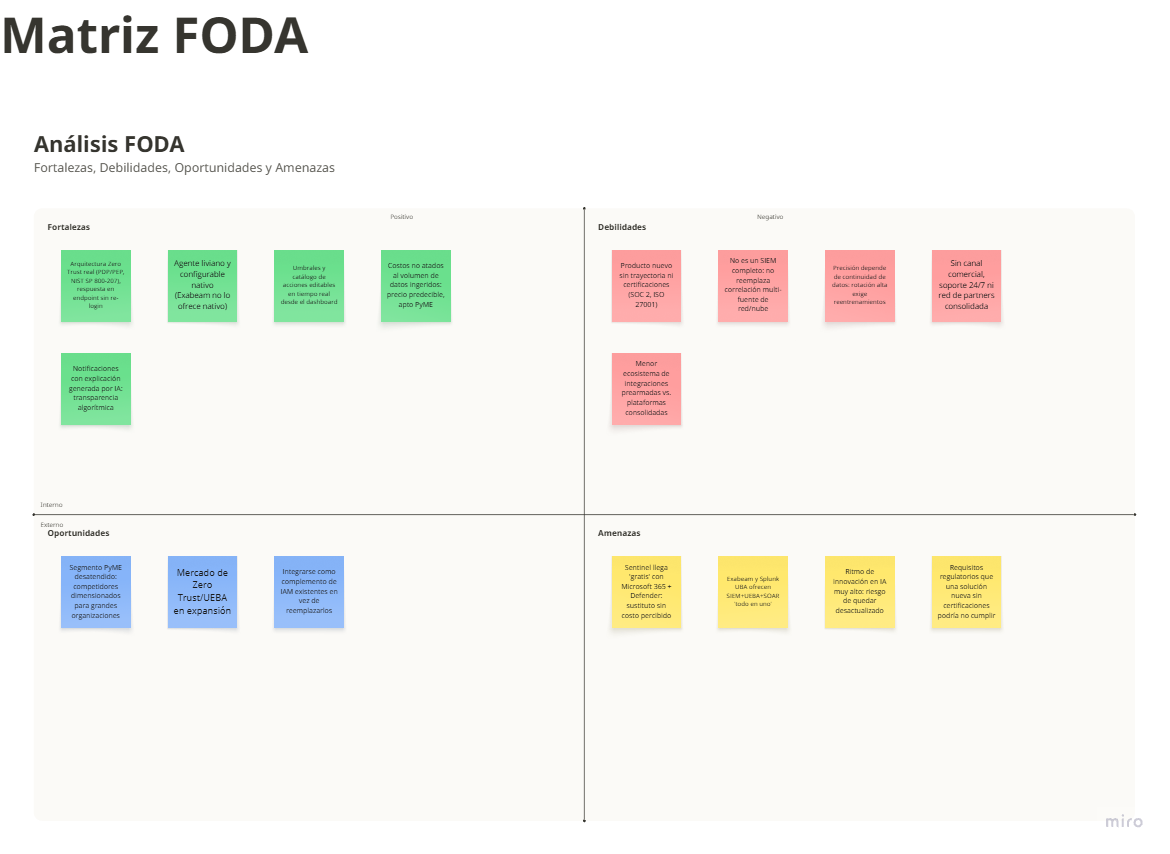
\includegraphics[width=\textwidth]{images/diagramas/Analisis_FODA.png}
	\caption{Matriz FODA del producto.}
	\label{fig:matriz-foda}
	{\small Fuente: elaboración propia.\par}
\end{figure}
\FloatBarrier

\subsection{Fortalezas}
Las fortalezas son factores internos que favorecen al producto frente a las soluciones relevadas:
\begin{itemize}
	\item Arquitectura basada en la separación entre punto de decisión y punto de aplicación de NIST SP~800-207, con respuesta ejecutada en el \emph{endpoint} sin \emph{re-login}: cierra el punto ciego que el propio Estado del arte identifica como carencia común de Sentinel, Splunk UBA y Exabeam.
	\item Agente liviano y configurable nativo, algo que Exabeam no ofrece de forma nativa.
	\item Umbrales y catálogo de acciones editable en tiempo real desde el \emph{dashboard}, sin depender de integraciones externas como sí necesita Splunk UBA.
	\item Modelo de costos no atado al volumen de datos ingeridos (a diferencia de Sentinel), lo que permite un precio predecible y bajo, acorde al presupuesto de una PyME.
	\item Una notificación que informa las variables que más contribuyen a cada alerta, redactada en forma opcional por un modelo de lenguaje, atendiendo la falta de transparencia algorítmica que el Estado del arte señala en Sentinel.
\end{itemize}

\subsection{Debilidades}
Las debilidades son factores internos que limitan al producto frente a esas mismas soluciones:
\begin{itemize}
	\item Producto nuevo en el mercado, sin trayectoria ni certificaciones (SOC 2, ISO 27001) que sí tienen Sentinel, Splunk UBA y Exabeam: la confianza institucional se construye con tiempo, no solo con calidad técnica.
	\item No es un SIEM completo: se enfoca en el comportamiento del usuario en el \emph{endpoint}, no reemplaza la correlación multi-fuente de eventos de red/nube que sí ofrecen los tres competidores.
	\item La precisión del modelo depende de la continuidad de los datos de comportamiento de cada usuario: alta rotación de personal o cambios de rol frecuentes exigen reentrenamientos más seguidos.
	\item Sin canal comercial, soporte 24/7 ni red de \emph{partners} consolidada desde el lanzamiento, algo que Sentinel, Splunk UBA y Exabeam ya tienen resuelto por años de estar en el mercado.
	\item Menor ecosistema de integraciones prearmadas con otras herramientas de seguridad, comparado con plataformas consolidadas con años de desarrollo de \emph{partners}.
\end{itemize}

\subsection{Oportunidades}
Las oportunidades son factores externos del mercado que el producto puede aprovechar:
\begin{itemize}
	\item Segmento PyME desatendido: las tres soluciones relevadas están dimensionadas y tarifadas para organizaciones grandes con equipo de seguridad dedicado.
	\item Mercado de Zero Trust/UEBA en expansión.
	\item Posibilidad de integrarse como complemento de soluciones IAM existentes, mediante el adaptador de identidad, hoy validado con un proveedor simulado, en vez de competir por reemplazarlas.
\end{itemize}

\subsection{Amenazas}
Las amenazas son factores externos que pueden dificultar la adopción del producto:
\begin{itemize}
	\item Sentinel se percibe como incluido para quien ya contrata Microsoft 365 con Defender: un sustituto sin costo adicional.
	\item Exabeam y Splunk UBA, al integrar SIEM+UEBA+SOAR, pueden ofrecerse como solución ``todo en uno'' frente a un producto que hoy resuelve una sola capa.
	\item Ritmo de innovación muy alto en IA aplicada a seguridad: riesgo de quedar desactualizado sin inversión continua.
	\item Requisitos regulatorios/de \emph{compliance} que una solución nueva sin certificaciones podría no cumplir en una primera etapa.
\end{itemize}

\section{Cruz de Porter: 5 fuerzas}
El análisis sigue el modelo de las cinco fuerzas competitivas \parencite{Porter1979}, aplicado al segmento elegido.

\begin{enumerate}
	\item \textbf{Rivalidad entre competidores existentes, alta en el segmento \emph{enterprise}, baja en el segmento elegido.} Sentinel, Splunk UBA y Exabeam compiten entre sí por el cliente grande; ninguno de los tres está diseñado ni tarifado para el segmento PyME, por lo que en ese segmento la rivalidad directa es baja.
	\item \textbf{Amenaza de nuevos competidores, media.} La barrera técnica (modelos de comportamiento confiables) es real, pero la infraestructura \emph{cloud} abarata el costo de entrada. El crecimiento del mercado Zero Trust también atrae nuevos entrantes.
	\item \textbf{Amenaza de productos sustitutos, alta.} El sustituto más directo no es otro UEBA, sino mantener la situación actual y continuar con Sentinel, ya incluido en una suscripción de Microsoft 365 existente, aunque tenga las limitaciones de costo por volumen y opacidad que señala el propio Estado del arte.
	\item \textbf{Poder de negociación de los compradores, alto en \emph{enterprise}, más bajo en PyME.} Las grandes organizaciones tienen alternativas consolidadas (Sentinel, Splunk, Exabeam) y capacidad de negociar. El comprador PyME hoy no tiene una alternativa dedicada a su tamaño entre estas tres, lo que da más previsibilidad al posicionamiento propuesto.
	\item \textbf{Poder de negociación de los proveedores, medio.} Dependencia de servicios \emph{cloud} gestionados (Redis, Postgres, API de Gemini) reemplazables sin bloquear el producto. El \emph{dataset} de entrenamiento (CLUE-LDS) es de acceso definido para el proyecto, no depende de un proveedor comercial de datos.
\end{enumerate}

\section{Matriz Boston Consulting Group (BCG)}
Con un único producto, la matriz \parencite{Henderson1970} se usa para posicionarlo dentro de su mercado, cruzando crecimiento del mercado vs.\ participación relativa. La Figura~\ref{fig:matriz-bcg} muestra la posición resultante del producto.

\begin{figure}[h]
	\centering
	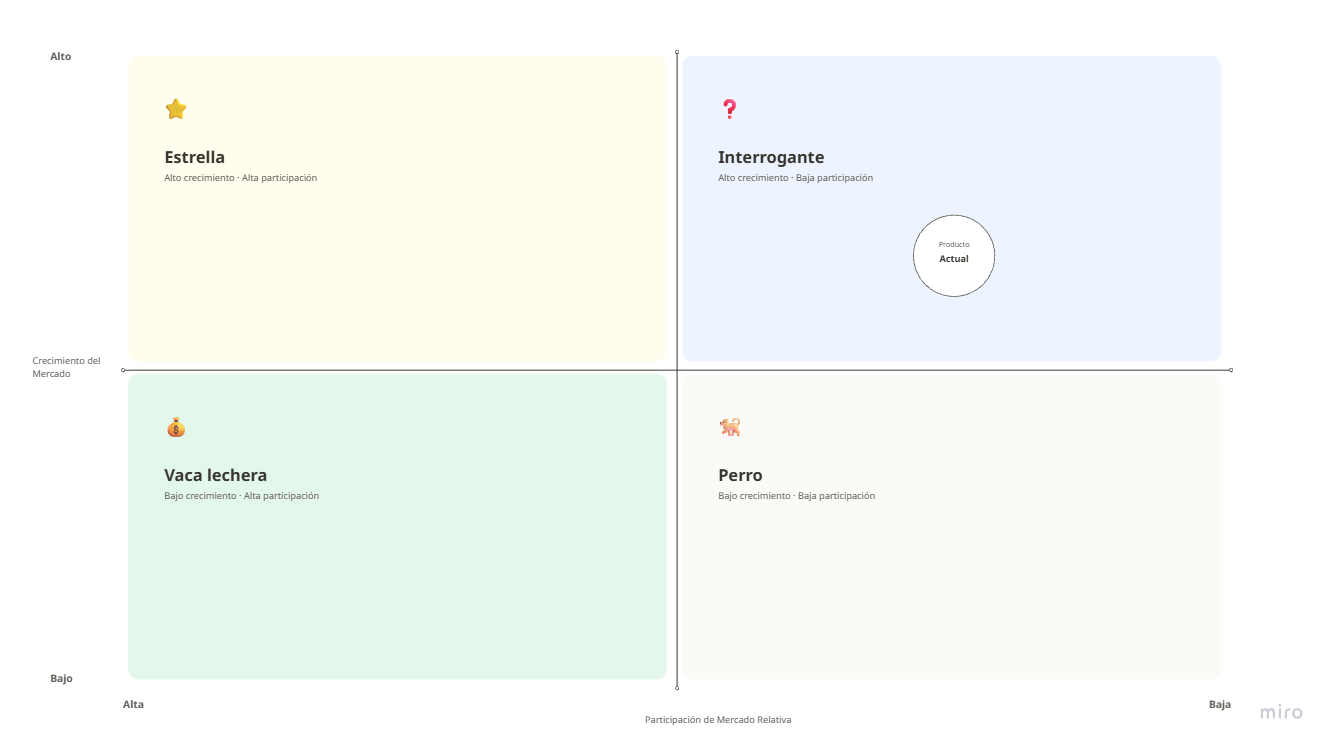
\includegraphics[width=\textwidth]{images/diagramas/BCG.png}
	\caption{Matriz Boston Consulting Group (BCG) del producto.}
	\label{fig:matriz-bcg}
	{\small Fuente: elaboración propia.\par}
\end{figure}
\FloatBarrier

\begin{itemize}
	\item \textbf{Eje crecimiento del mercado: alto.} Se ubica en el extremo alto por dos motivos. Primero, un cambio estructural: el trabajo remoto y la migración a servicios en la nube reducen la eficacia de la seguridad perimetral, premisa de la que parte el enfoque Zero Trust \parencite{Rose2020}, y obligan a controlar la actividad posterior al inicio de sesión (sección~\ref{sec:punto-ciego}). Segundo, la literatura sobre UEBA y control de acceso adaptativo relevada en el estado del arte es en su mayoría reciente, lo que indica un campo en desarrollo activo. La valoración es cualitativa: el proyecto no cuenta con datos propios sobre el tamaño ni la tasa de crecimiento del mercado.
	\item \textbf{Eje participación relativa de mercado: baja.} La participación relativa se mide contra el líder del segmento. Las tres soluciones relevadas tienen una posición consolidada: Sentinel se distribuye integrado al ecosistema de Microsoft, Splunk tiene una trayectoria extensa en el mercado de SIEM y Exabeam combina capacidades de SIEM, UEBA y SOAR. El producto, en cambio, no tiene clientes, marca reconocida ni implementaciones previas, por lo que su participación inicial es nula. La participación se construye con tiempo de operación en el mercado y no depende solo de la calidad técnica del producto.
\end{itemize}

Interrogante / Dilema (\emph{Question Mark}). Mercado de alto crecimiento donde el producto todavía no tiene participación, por lo que requiere inversión para intentar moverse hacia el cuadrante ``Estrella''. La estrategia recomendada para este cuadrante es la seguida en el posicionamiento: no competir de frente contra Sentinel, Splunk UBA y Exabeam en su propio segmento (\emph{enterprise}), sino ganar adopción en el corto plazo en el nicho PyME que esas tres soluciones dejan desatendido por su modelo de costos e implementación.

\clearpage
